%% Copernicus Publications Manuscript Preparation Template for LaTeX Submissions
%% ---------------------------------
%% This template should be used for copernicus.cls
%% The class file and some style files are bundled in the Copernicus Latex Package, which can be downloaded from the different journal webpages.
%% For further assistance please contact Copernicus Publications at: production@copernicus.org
%% https://publications.copernicus.org/for_authors/manuscript_preparation.html

%% copernicus_rticles_template (flag for rticles template detection - do not remove!)

%% Please use the following documentclass and journal abbreviations for discussion papers and final revised papers.

%% 2-column papers and discussion papers
\RequirePackage[2020/02/02]{latexrelease}
\documentclass[gc, manuscript]{copernicus}



%% Journal abbreviations (please use the same for discussion papers and final revised papers)


% Advances in Geosciences (adgeo)
% Advances in Radio Science (ars)
% Advances in Science and Research (asr)
% Advances in Statistical Climatology, Meteorology and Oceanography (ascmo)
% Annales Geophysicae (angeo)
% Archives Animal Breeding (aab)
% ASTRA Proceedings (ap)
% Atmospheric Chemistry and Physics (acp)
% Atmospheric Measurement Techniques (amt)
% Biogeosciences (bg)
% Climate of the Past (cp)
% DEUQUA Special Publications (deuquasp)
% Drinking Water Engineering and Science (dwes)
% Earth Surface Dynamics (esurf)
% Earth System Dynamics (esd)
% Earth System Science Data (essd)
% E&G Quaternary Science Journal (egqsj)
% European Journal of Mineralogy (ejm)
% Fossil Record (fr)
% Geochronology (gchron)
% Geographica Helvetica (gh)
% Geoscience Communication (gc)
% Geoscientific Instrumentation, Methods and Data Systems (gi)
% Geoscientific Model Development (gmd)
% History of Geo- and Space Sciences (hgss)
% Hydrology and Earth System Sciences (hess)
% Journal of Bone and Joint Infection (jbji)
% Journal of Micropalaeontology (jm)
% Journal of Sensors and Sensor Systems (jsss)
% Magnetic Resonance (mr)
% Mechanical Sciences (ms)
% Natural Hazards and Earth System Sciences (nhess)
% Nonlinear Processes in Geophysics (npg)
% Ocean Science (os)
% Primate Biology (pb)
% Proceedings of the International Association of Hydrological Sciences (piahs)
% Scientific Drilling (sd)
% SOIL (soil)
% Solid Earth (se)
% The Cryosphere (tc)
% Weather and Climate Dynamics (wcd)
% Web Ecology (we)
% Wind Energy Science (wes)


%% \usepackage commands included in the copernicus.cls:
%\usepackage[german, english]{babel}
%\usepackage{tabularx}
%\usepackage{cancel}
%\usepackage{multirow}
%\usepackage{supertabular}
%\usepackage{algorithmic}
%\usepackage{algorithm}
%\usepackage{amsthm}
%\usepackage{float}
%\usepackage{subfig}
%\usepackage{rotating}

% Pandoc citation processing

% The "Technical instructions for LaTex" by Copernicus require _not_ to insert any additional packages.
%
\usepackage{algorithmic}
\usepackage{algorithm}


\begin{document}

\title{Management induced changes of soil organic carbon on global croplands}


\Author[1]{Kristine}{Karstens}
\Author[1]{Benjamin Leon}{Bodirsky}
\Author[2]{Your}{Name}
\Author[1]{Alexander}{Popp}


\affil[1]{Potsdam-Institut of Climate Impacts Research, Potsdam, Germany}
\affil[2]{Your affiliation}

\runningtitle{R Markdown Template for Copernicus}

\runningauthor{Nüst et al.}


\correspondence{Kristine\ Karstens\ (\href{mailto:kristine.karstens@pik-potsdam.de}{\nolinkurl{kristine.karstens@pik-potsdam.de}})}



\received{}
\pubdiscuss{} %% only important for two-stage journals
\revised{}
\accepted{}
\published{}

%% These dates will be inserted by Copernicus Publications during the typesetting process.


\firstpage{1}

\maketitle


\begin{abstract}
Soil organic carbon (SOC) is one of larges carbon stocks on Earth. It is three times larger than the vegetation pool and more than twice as big as the athmospheric pool, when looking into the first meter of the earth soil profile. Human cropping activties led and still lead to a depletion of SOC though, which are so far not well represented in global assessments of historic carbon emissions. While SOC models often represent well the biochemical processes that lead to the accumulation and decay of SOC, the management decisions driving these biophysical processes are still little investigated on the global scale. Here we create a spatial explicit data set for agricutural management on cropland, especially for crop residue and manure management, based on global historic production (FAOSTAT), and land-use (LUH2) data; and combine it with the IPCC Tier 2 approach to create a half degree resolution SOC stock changes on mineral soils. We estimate that due to arable farming soils have lost over 37 GtOC of which 4 GtOC have been regained within the period 1975-2010. We show that, our results on global scale based on Tier 2 IPCC methodolgy are in good agreement with Tier 1 default assumptions. We also find that SOC is very sensitive to management decision such as residue recycling indicating the nessessity to incorporated better management data in soil models.
\end{abstract}


\copyrightstatement{The author's copyright for this publication is transferred to institution/company.}


\newpage

\introduction

Soil Organic Carbon (SOC), the amount of organic carbon stored through the earth's soil, is the largest terrestrial carbon pool, exceeding the carbon in the atmospheric and vegetation pools multiple times (Batjes). As such, even small changes in drivers of SOC may thus lead to substantial shifts in earth carbon cycle and influence the amount of CO2 in the atmosphere (ref. permafrost melting). The specific amount of carbon stored in the soil is, however, uncertain, with estimates ranging from 1500 to 2400 GtC for the first meter of the soil profile (Batjes, 1996; more). The quality of SOC maps has markedly improved in recent decades, along with better understanding of the factors driving the global magnitude, distribution, and dynamics of SOC pools. Natural properties like climatic, biophysical, and landscape characteristics clearly play the most important roles to determine SOC variations over space and time.
Human intervention, including land cover change and land management, has however added a further driver to SOC change, which alters terrestrial carbon pools over much shorter time scales and is likely one of the most dominant driver of SOC changes on managed land today (cite). Recent studies identify the anthropogenic SOC debt for the first meter of the soil profile at around 116 GtC (Sanderman et al.), compared to previous estimates between 60-130 GtC (Lal, 2006). Other studies have focused more closely on spatially disaggregation of SOC changes via advanced digital soil mapping techniques (S-World; Stoorvogel 2, 2017) or better representation of biogeochemical processes within SOC dynamics (Hararuk, 20XX). While providing a rough estimate of the order of magnitude of change, these studies lack a detailed consideration of land management, especially of agricultural activities.
Field-scale models (cite Daycent, RothC, Ecosse, C-Tool) are able to capture these land management impacts by using detailed information on crop yield levels, fertilizer inputs and various other on-farm measures. However, due to the lack of comprehensive global management data as input to these models, scaling up to the global extent remains a complex challenge. Our study combines a spatially explicit estimate of agricultural management data on the global level with a 3-pool SOC model parametrized for global croplands. This allows us to estimate SOC stock change factors, as well as organic carbon flow dynamics within the agricultural system. We thereby consider change in SOC caused by historical land cover change as well as of different agricultural management practices, including residue recycling, manure amendments, irrigation, and tillage. We provide the first global, spatially explicit SOC loss maps that considers detailed agricultural management.
This paper will first introduce in the methods section the basic concept of SOC dynamics as applied in this study. Additionally, we shortly refer to the concept of stock change factors as outlined in the Tier 1 approach of the IPCC guidelines. Lastly, we continue with a detailed description of the global gridded management data used here, including crop production levels, residue recycling rates, manure amendments, and the adoption of irrigation and tillage practices. In our results section we focus on the SOC dynamics of global croplands by (1) analysing the spatially explicit distribution and depletion of SOC from 1975 to 2010, (2) comparing impacts of different management effects on SOC emissions and (3) quantify global agricultural carbon flows and stocks to compare the importance of various management aspects. Finally, we discuss and compare our findings -- including their implications for SOC model development -- and conclude with an outlook on the ability of SOC management to mitigate climate change and contribute to negative greenhouse gas emissions.
\newpage

\hypertarget{method}{%
\section{Method}\label{method}}

We compile calculations as open-source R packages available at github.com/pik-piam/mrcommons (management related functions) and github.com/pik-piam/mrSOCbudget (soil dynamic related functions), which are both based on the MADRaT package (package citation?), a framework which aims to improve reproducibility and transparency in data processing.
In the following section we outline the most important relationships and assumptions. Table \ref{append:subsection2mrfunctions} provides further information on corresponding code within the R packages.

\hypertarget{sec:carbonbudget}{%
\subsection{SOC Stocks and Stock changes following the Tier 2 steady-state method}\label{sec:carbonbudget}}

Following the tier 2 approach of the refinement of IPCC guidelines vol.~4 (\citet{ipcc_2019_2019}; short Tier 2 steady-state method), we estimate soil organic carbon (SOC) stocks and their change over time for cropland on half-degree resolution from 1975 to 2010. We assume the current SOC state converges towards a steady state, which itself is depending on biophysical, climatic and agronomic conditions. Therefore, we conduct the following three steps within each yearly time-step:
(1) We calculate annual land-use (sub-)type-specific steady states and decay rates for SOC stocks,
(2) we account for land conversion by transferring SOC from and to another land-use type represented as natural vegetation,
(3) we estimate SOC stocks and changes based on the stocks of the previous time period, the steady state stocks and the decay rate.

\hypertarget{steady-state-soc-stocks-and-decay-rates}{%
\subsubsection{Steady-state SOC stocks and decay rates}\label{steady-state-soc-stocks-and-decay-rates}}

In a simple first order kinetic approach the steady-state soil organic carbon stocks \(SOC^{eq}\) are given by
\begin{equation}
SOC^{eq} =\frac{C^{\textrm{in}}}{k} \qquad\forall\quad i,t
\label{eq:inoutflow}
\end{equation}
with \(C^{\textrm{in}}\) being carbon inputs to the soil, \(k\) denoting the soil organic carbon decay rate; as well as \(i\) representing grid cell identifier and \(t\) years. We use for our calculations the Tier 2 steady-state method, which assumes three soil carbon sub-pools (active, slow and passive) and interactions between them, following the approach in the Century model (Parton et al, 1988). Annual carbon inflow to each sub-pool and annual decay rates of each sub-pool are the key components to determining steady-state SOC stocks.

\textbf{Carbon Inputs to the Soil}

We account for different carbon input sources depending on the two land-use types we distinguish: croplands and natural vegetated land as representative for all other land use (see table \ref{tab:datasourceinputs}). Carbon sources for cropland are recycled crop residues, below ground biomass of crops (for both see \ref{sec:residues}) and recycled manure (see \ref{sec:livstmanure}); for natural vegetation litterfall (including fine root turnover) \citep{schaphoff_lpjml4_2018} is the only source of carbon inflow to the soil.

Following the IPCC carbon accounting methodology, carbon inputs are disaggregated into metabolic and structural components depending on their lignin and nitrogen content (see \citet{ipcc_2019_2019}). For each component the sum of all carbon input sources is allocated to the respective SOC sub-pools via transfer coefficients. This implies that both the amount of carbon and its structural composition determine the effective inflow. Data sources for all considered carbon inputs as well as for lignin and nitrogen content can be found in table \ref{tab:datasourceinputs}.

 \begin{table*}[h]
 \caption{Type and data sources for carbon inputs to different land-use types }
 \begin{tabular}{l l l l}
 \tophline
  \textbf{land-use types}   & \textbf{source of carbon inputs} & \textbf{data source} & \textbf{nitrogen and lignin content} \\
 \middlehline
 \multirow{3}{*}{Cropland} & residues & FAOSTAT, LPJmL4 [2, sec:residues] & default values given by [2]  \\
                            & dead below ground biomass of crops & FAOSTAT, LPJmL4 [2, sec:residues] & default values given by [2] \\
                            & manure & FAOSTAT, Isabelle [2, sec:manure] & default values given by [2] \\
                            \hline
  Natural vegetation        & annual litterfall & LPJmL4 [4]& \begin{minipage}[t]{0.28\columnwidth}\raggedright\strut Nitrogen and lignin content of tree compartments used in CENTURY [4] \strut \end{minipage}\tabularnewline
 \bottomhline
 \end{tabular}
 \label{tab:datasourceinputs}
 \belowtable{}
 \end{table*}

\textbf{SOC decay}

The sub-pool specific decay rates are influenced by climatic conditions, biophysical and biochemical soil properties as well as management factors that all vary over time (t) and space (i). Following the Tier 2 steady-state method we consider temperature (temp), water (wat), sand fraction (sf) and tillage (till) effects to account for spatial variation of decay rates. Thus, \(k_{sub}\) is given by

\begin{equation}
\begin{aligned}
& k_{active,t,i}  & = &~ k_{active}  ~ &\cdot~ temp_{t,i} ~ &\cdot~ wat_{t,i} ~ &\cdot~ till_{t,i} ~ & \cdot~ sf_{t,i}\\
& k_{slow,t,i}    & = &~ k_{slow}    ~ &\cdot~ temp_{t,i} ~ &\cdot~ wat_{t,i} ~ &\cdot~ till_{t,i} ~ &\\
& k_{passive,t,i} & = &~ k_{passive} ~ &\cdot~ temp_{t,i} ~ &\cdot~ wat_{t,i} ~ & ~ &
\label{eq:decayrates}
\end{aligned}
\end{equation}

For cropland, we distinguish the effect of different tillage (see \ref{sec:tillage}) and irrigation (see \ref{sec:irrigation}) practices on decay rates, whereas for natural vegetation, we assume rainfed and non-tilled conditions. Data sources as well as drivers considered for each land-use types are shown in table \ref{tab:datasourcedecay}. To account for variations of decay rates within each grid cell due to different tillage and irrigation regimes, average rates based on area shares are calculated.

 \begin{table*}[h]
 \caption{Type and data sources for carbon inputs to different land-use types}
 \begin{tabular}{l l l l}
 \tophline
  land-use types   & type of decay driver & parameter use to represent driver & data source \\
 \middlehline
 \multirow{2}{*}{all} & Soil quality & Sand fraction of the first 0-30 cm &  [SoilGrids]  \\
                      \cline{2-4}
                      
                      & Mircobial activity & air temperature & [CRUp4.0] \\
                      \cline{2-4}
                      
                      & Water restriction & precipitation \& potential evapotranspiration & [CRUp4.0] \\
                      \cline{1-4}
\multirow{2}{*}{\begin{minipage}[t]{0.2\columnwidth}\raggedright\strut Cropland\\(additionally)\strut\end{minipage}} & Water restriction*  & irrigation  & [sec:irrigation] \\ 
                      \cline{2-4}
                      
                      & Soil disturbance & tillage & [sec:tillage] \\
 \bottomhline
 \end{tabular}
 \belowtable{}
 \label{tab:datasourcedecay}
 \end{table*}

\hypertarget{soc-transfer-between-land-use-types}{%
\subsubsection{SOC transfer between land-use types}\label{soc-transfer-between-land-use-types}}

We calculate SOC stocks based on the area shares of land-use types (lut) within the half-degree grid cells (i). If land is converted from one land-use type into others (!lut), the respective share of the SOC stocks is reallocated. We account for land conversion at the beginning of each time step \(t\) by calculating a preliminary stock \(SOC_{lut,t*}\) via

\begin{equation}
SOC_{lut,t*} = SOC_{lut,t-1} - \frac{SOC_{lut,t-1}}{A_{lut,t-1}} \cdot  AR_{lut,t} + \frac{SOC_{!lut,t-1}}{A_{!lut,t-1}} \cdot  AE_{lut,t} \qquad \forall\quad sub, i  
\label{eq:ctransfer}
\end{equation}

with \(A\) being the area, \(AR\) the area reduction and \(AE\) the area expansion for a given land-use type \(lut\). Note that \(!lut\) denotes the sum over all other land-use types, which decreases in the specific time step \(t\). Data sources and methodology on land-use states and changes are described in \ref{sec:landuse}.

\hypertarget{total-soc-stocks-and-stock-changes}{%
\subsubsection{Total SOC stocks and stock changes}\label{total-soc-stocks-and-stock-changes}}

Carbon stocks \(SOC\) for each sub-pool (sub) converge towards the calculated steady-state stock \(SOC^{eq}\) for each land-use type (lut), each sub-pool (sub) and each annual time step (t) like

\begin{equation}
SOC_{t} = SOC_{t-1} + (SOC^{eq}_{t} - SOC_{t-1}) \cdot k_{t} \cdot 1\unit{a} \qquad \forall\quad\quad lut, sub, i.
\label{eq:SOCstate}
\end{equation}

Reformulating this equation, we obtain a mass balance equation as follows

\begin{equation}
SOC_{t} = SOC_{t-1} - \underbrace{SOC_{t-1} \cdot k_{t} \cdot 1\unit{a}}_{\text{outflow}} + \overbrace{SOC^{eq}_{t} \cdot k_{t} \cdot 1\unit{a}}^{\text{input (using equation (1))}}  \qquad \forall\quad lut, sub, i.
\label{eq:steadystate2budget}
\end{equation}

The global SOC stock for each time step can then be calculated via

\begin{equation}
SOC_{t} = \sum_{i} \underbrace{\sum_{lut} \overbrace{\sum_{sub} SOC_{lut, sub, t, i}.}^{\text{$SOC_{lut, t, i}$ -- land-use type specific SOC stock within cell}}}_{\text{$SOC_{t, i}$ -- total SOC stock within cell}}
\label{eq:totalstock}
\end{equation}

According to the IPCC guidelines SOC changes can be expressed as the difference of two consecutive years (see Eq. 5.0A in \citep{ipcc_2019_2019}). This however, will also include naturally occurring changes due to climatic variance over time. For our study we defined the absolute and relative SOC changes in relation to a potential natural state \(SOC_{pnv}\) under the same climatic conditions at time \(t\) in grid cell \(i\), that is based on the natural vegetation SOC calculations as defined above without accounting for land conversion from cropland at any time. The absolute changes \(\Delta SOC\) and relative changes \(F^{SCF}\) a thus given by

\begin{equation}
\Delta SOC_{t, i} = SOC_{t, i} - SOC_{pnv, t, i}\quad, \qquad \quad  F^{SCF}_{t, i} = \frac{SOC_{t, i}}{SOC_{pnv, t, i}}.
\label{eq:stockdiff}
\end{equation}

Note that the absolution changes \(\Delta SOC\) can be also interpreted as the SOC gap due to human cropping activities; whereas relative changes \(F^{SCF}\) can be denoted as stock change factors as defined within the IPCC guidelines of 2006 \citep{ipcc_2006_2006}. Note that the SOC gap is equivalent to the negated cumulative SOC emission (\citep{pugh_simulated_2015}) also referred to as SOC debt (\citep{sanderman_soil_2017}) of human land use.

\hypertarget{initialization-of-soc-pools}{%
\subsubsection{Initialization of SOC pools}\label{initialization-of-soc-pools}}

To initialize all SOC sub-pools we assume that cropped land as well as natural vegetation are in a steady state for the specific configuration present within the initialization year 1961. We assume after a spin-up period of 15 years reliable results start from 1975 and improve over time, since dependency on the initial conditions decreases.

\hypertarget{sec:tier1}{%
\subsection{SOC Stocks and Stock changes following Tier 1}\label{sec:tier1}}

Additionally, to the tier 2 approach of the refinement of IPCC guidelines vol.~4 \citep{ipcc_2019_2019} and the detailed analysis of management data coming with it, SOC changes can be estimated using the IPCC tier 1 approach of IPCC guidelines vol.~4 (\citet{ipcc_2006_2006}, \citet{ipcc_2019_2019}). Here, stocks are calculated via stock change factors (\(F^{SCF}\)) given by the IPCC for the topsoil (0-30 cm) and based on observational data. \(F^{SCF}\) are differentiated by different crop, management and input systems (here summarized under \(m\)) reflecting different dynamics under changed in- and outflows without explicitly tracking these. Moreover, \(F^{SCF}\) vary for different climatic zones (\(c\)) specified by the IPCC (see \ref{append:climatemap}). The actual SOC stocks as thus calculated based on a given reference SOC stock by

\begin{equation}
SOC^{\text{target}}_{i} = \sum_{c,m} T_{c,i} \cdot SOC^{\text{ref}} \cdot F^{SCF}_{c,m} \qquad\forall\quad t,
\label{eq:tier1}
\end{equation}

with \(T_{c,i}\) being the translation matrix for grid cells \(i\) into corresponding climate zones \(c\). For this analysis we use the default \(F^{SCF}\) from the Tier 1 method of \citep{ipcc_2006_2006}, and \citep{ipcc_2019_2019} as a comparison and consistency check for our more detailed budget approach.

\newpage

\hypertarget{sec:agrimanagement}{%
\subsection{Agricultural management data on 0.5 degree resolution}\label{sec:agrimanagement}}

We compile country-specific FAO production and cropland statistics \citep{faostat_faostat_2016} to a harmonized and consistent data set. The data is prepared in 5 year time steps from 1965 to 2010, which, together with the spin up phase, restricts our analysis to time span from 1975 to 2010. For all the following data, if not declared differently, we interpolate values linearly between the time steps and hold them constant before 1965.

\hypertarget{sec:landuse}{%
\subsubsection{Land use and Land-use change}\label{sec:landuse}}

Land-use patterns are based on the Land-Use Harmonization 2 \citep{hurtt_harmonization_2020} data set, which we aggregate from quarter degree to half degree resolution. We disaggregate the five different cropland subcategories (c3ann, c3per, c4ann, c4per, c3nfx) of LUH2 into our 17 crop groups, applying the relative shares for each grid cell based on the country and year specific area harvested shares of FAOSTAT data \citep{faostat_faostat_2016} (see \ref{append:Tableluh2fao2mag} for more details on the crop group mapping). Land-use transitions are calculated as net area differences of the land-use data on half-degree.

\hypertarget{sec:residues}{%
\subsubsection{Crop and Crop Residues Production}\label{sec:residues}}

\textbf{Crop Production}

Using half-degree yield data from LPJmL \citep{schaphoff_lpjml4_2018} as well as half-degree cropland patterns (see \ref{sec:landuse}) we compile crop group specific half-degree production patterns. We calibrate cellular yields with a country-level calibration factor for each crop group to meet historical FAOSTAT production \citep{faostat_faostat_2016}. Note that by using physical cropland areas we account for multiple crop harvest events as well as for fallows.

\textbf{Crop Residue Production}

Crop residue production and management is based on a revised methodology of \citep{bodirsky_n2o_2012} and key aspects are explained here given its central role for soil carbon modelling. Starting from harvested crop production (\(CP\)) estimates and their respective harvested crop area (\(CA\)), we estimate above-ground (\(AGR\)) and below-ground (\(BGR\)) residual biomass using crop group (\(cg\)) specific harvest index values (\(HI\)) and root:shoot ratios (\(RS\)) as follows

\begin{equation}
\begin{aligned}
AGR & = CP \cdot HI_{\textrm{slope}} + CA \cdot HI_{\textrm{intercept}}\qquad & \textrm{and} \\
BGR & = (CP + AGR) \cdot RS \qquad                                            & \forall\quad cg, i, t.
\label{eq:resbiomass}
\end{aligned}
\end{equation}

Following the IPCC guidelines, we split the harvest index into a yield and an area dependent fraction \citep{ipcc_2006_2006}. Note that deviating from \citep{bodirsky_n2o_2012} we use harvested instead of physical crop area to account for increased residue biomass due to multiple cropping and decreased amounts on fallow land.
We assume that all BGR are recycled to the soil, whereas AGR can be burned or harvested for other purposes such as feeding animals \citep{weindl_livestock_2017}, fuel or for material use.

\textbf{Burned Residues}

A fixed share of the AGR is assumed to be burned on field depending on the per-capita income of the country. Following \citep{smil_nitrogen_1999}) we assume 25\% burn share for low-income countries according to World Bank definitions (\(<\,1000\,\tfrac{USD}{yr\,cap}\)), 15\% for high-income (\(>\,10000\,\tfrac{USD}{yr\,cap}\)) and linearly interpolate shares for all middle-income countries depending on their per-capita income. Depending on the crop group 80--90\% of the residue carbon burned on the fields are lost within the combustion process \citep{ipcc_2006_2006}.

\textbf{Residue Usage}

We compile out of our 17 crop groups, three residue groups (straw, high-lignin and low-lignin residues) with additional demand for other purposes and one residue with no double use (see \ref{append:Tablekcr2kres}). Residue feed demand for five different livestock groups is based on country- and residue-group-specific feed baskets (see \citep{weindl_livestock_2017}), taking available AGR biomass as well as livestock productivity into account. We estimate, for low-income countries, a material-use share for straw residues of 5\% and a fuel-share of 10\% for all used residues groups in low-income countries. For high-income countries, no withdrawal for material or fuel use is assumed, and middle-income countries use shares are linearly interpolated based on per-capita income. The remaining AGR as well as all BGR are expected to be recycled to the soil. We limit high recycling shares at \(10\tfrac{\unit{tC}}{\unit{ha}}\) to correct for outliers.

\textbf{Dry Matter to Carbon Transformation}

To transform dry matter estimates into carbon, we compiled crop-group and plant part specific carbon to dry matter (c:dm) ratios (see \ref{append:Tablec2dm}).

\hypertarget{sec:livstmanure}{%
\subsubsection{Livestock Distribution and Manure Excretion}\label{sec:livstmanure}}

We assume that manure is applied at its excretion place, leaving the livestock distribution the driving factor for the spatial pattern of manuring.

\textbf{Livestock Distribution}
To disaggregate country level FAOSTAT livestock production values to the half-degree scale, we use the following rule-based assumptions, drawing from the approach of \citep{robinson_mapping_2014}, and uses feed basket assumptions based on a revised methodology from \citep{weindl_livestock_2017}. We differentiate between ruminant and monogastric systems, as well as extensive and intensive systems.
For ruminants, we assume that livestock is located where the production of feed occurs. We distinguish between grazed pasture, which is converted into livestock products from extensive systems; and all other (crop-based) feeds, which we consider to be consumed in intensive systems.
For poultry, egg and monogastric meat production we use the per-capita income of the country to divide between intensive and extensive production systems. For low-income countries, we assume extensive production systems. We locate them according to the share of built-up areas based on the idea that these animals are held in subsistence or small-holder farming systems with a high labor per animal ratio. Intensive production associated with higher income countries, is distributed within a country using again share of crop-based feed production, assuming that feed availability is the most driving factor for livestock location.

\textbf{Manure Excretion, Storage and Recycling}
Manure production and management is based on a revised methodology of \citep{bodirsky_n2o_2012} and is presented here due to its central role in soil carbon modelling. Based on the gridded livestock distribution we calculate excretions by estimating the nitrogen balance of the livestock system on the basis of comprehensive livestock feed baskets \citep{weindl_livestock_2017}, assuming that all nitrogen in protein feed intake, minus the nitrogen in the slaughter mass, is excreted. Carbon in excreted manure is estimated by applying fixed C:N ratios (given by \citep{ipcc_2019_2019}).
Depending on the feed system we assume manure to be handled in four different ways:
All manure originated from pasture feed intake is excreted directly to pastures and rangelands (pasture grazing), deducting manure collected as fuel. Manure fuel shares are estimated using IPCC default values \citep{ipcc_2006_2006}.
Whereas for low-income countries, we adopt a share of 25\% of crop residues in feed intake directly consumed and excreted on crop fields (stubble grazing), we do not consider any stubble grazing in high-income countries; middle-income countries see linearly interpolated shares depending on their per-capita income.
For all other feed items we assume the manure to be stored in animal waste management systems associated with livestock housing.
To estimate the carbon actually recycled to the soil, we account for carbon losses during storage and recycling shares in different animal waste management and grazing systems. Whereas we assume no losses for pasture and stubble grazing, we consider that the manure collected as fuel is not recycled. For manure stored in different animal waste management systems we compiled carbon loss rates partly depending on the nitrogen loss rates as specified in \citep{bodirsky_n2o_2012} (see \ref{append:TableclossAWMS}). We limit high application shares at \(10\tfrac{\unit{tC}}{\unit{ha}}\) to correct for outliers.

\hypertarget{sec:irrigation}{%
\subsubsection{Irrigation}\label{sec:irrigation}}

We use irrigation area shares to modify the water effect on decomposition by weighting the irrigated and rainfed water factors based on these shares. The LUH2v2 \citep{hurtt_harmonization_2020} data set provides irrigated fractions for their cropland subcategories. We apply aggregated area shares, leading to the same impact of irrigation on all of our crop groups. Moreover, we assume the irrigation effect to be present for all 12 months of a year in grid cells, that has been marked as irrigated.

\hypertarget{sec:tillage}{%
\subsubsection{Tillage}\label{sec:tillage}}

To account for the distribution of tillage to the three different tillage types specified by the IPCC -- full tillage, reduced tillage and no tillage --, we assume that all natural land and pastures are not tilled, whereas as default annual crops are under full and perennials under reduced tillage. Furthermore, we assume no tillage in cropland cells specified as no tillage cell based on the historic global gridded tillage data set from \citep{porwollik_generating_2018}. This data set is extended by to the period of 1974-2010 by combining country-level data on conservation agriculture area values from AQUASTAT (FAO, 2016) and LUH2 crop areas together with the methodology of \citep{porwollik_generating_2018} to identify potential no tillage cells.
\newpage

\hypertarget{results}{%
\section{Results}\label{results}}

We present simulation results of our SOC budget focusing on cropland areas for the year 2010 as well as global trends of SOC stock changes for the period from 1975 to 2010.

\hypertarget{soc-distribution-and-depletion}{%
\subsection{SOC distribution and depletion}\label{soc-distribution-and-depletion}}

\begin{figure}[H]
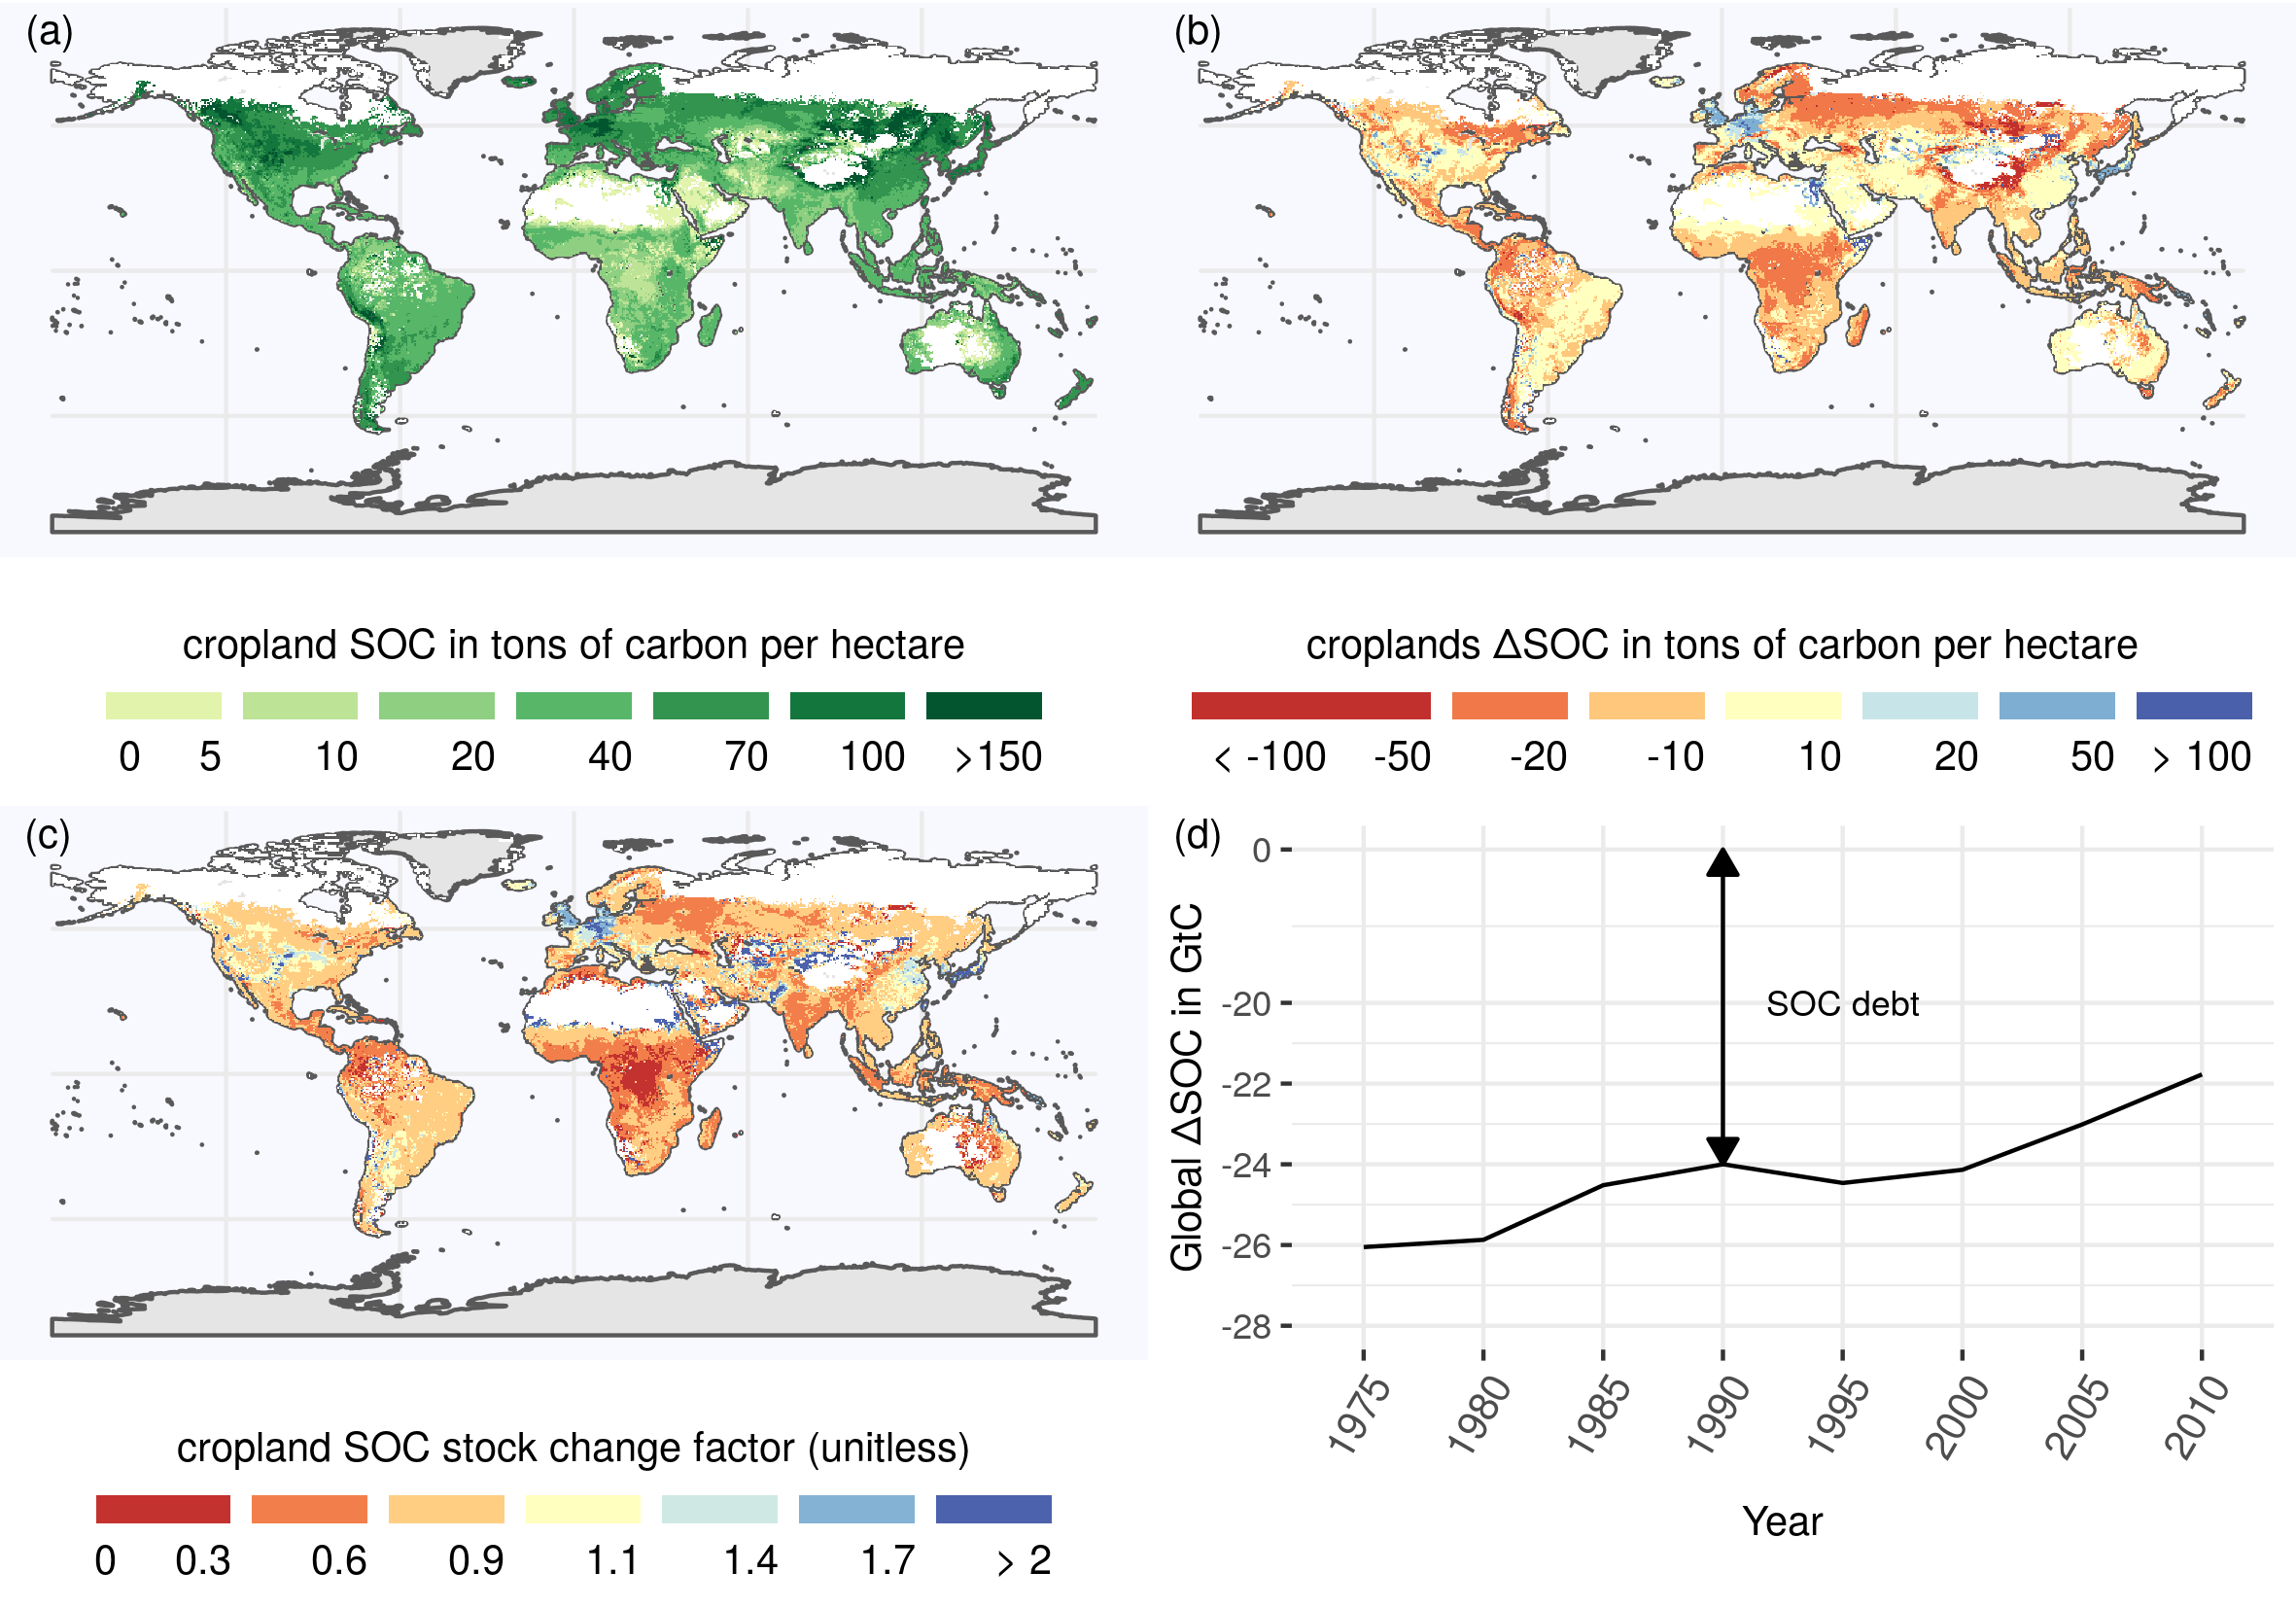
\includegraphics[width=18cm]{../ResultNotebooks/Output/Images/4panelfigure} \caption{(a): Distribution of total global SOC stocks on cropland shows high carbon stocks in high yielding areas. (b): The SOC debt is decreasing over time, meaning net SOC gains on global croplands over the last decades. (c)+(d): Absolute (c) and relative (d) SOC stocks compared to a potential natural state showing different hot spots of SOC dynamics. Whereas the absolute losses might be in temperate dry regions, relative losses are more prominent in tropical moist areas.}\label{fig:SOCmaps}
\end{figure}

In fig.~1(a) we provide the first world map of SOC on croplands considering real world management data on the global scale. Our spatially explicit results moreover show hot spots of SOC losses as well as gains in two different ways:
1. Absolute SOC changes (see fig.~1(c)) indicate areas with high importance for the global SOC emissions. The might be driven by huge relative losses or a high natural stock, from which even small deviations could lead to substantial losses.
2. To attribute SOC losses to insufficient agricultural management relative SOC changes (\(F^{SCF}\), see fig.~1(d)) are a helpful tool. They indicate areas with huge difference in carbon inflows or SOC decay compared to natural vegetation, that might be overcome due to improved agricultural practices.

\hypertarget{agricultural-management-effects-on-soc-emissions-and-cycling}{%
\subsection{Agricultural management effects on SOC emissions and cycling}\label{agricultural-management-effects-on-soc-emissions-and-cycling}}

Global cumulative SOC emissions are decreasing (see fig.~1(c)). Fig. 2 reveals the relative impact of management effects by freezing tillage areas as well as carbon inflows from residues or manure at the level of 1975. Our counterfactual scenarios show that the increasing residue carbon input had the biggest overall effect on SOC stocks. Without changes in management regimes especially in residue inflows to the soil, global cumulative SOC emissions would still grow. The strong effect of carbon residue amounts are also visible in the carbon flow diagram for agricultural production for the year 2010 (see fig.~3)

\begin{figure}[H]
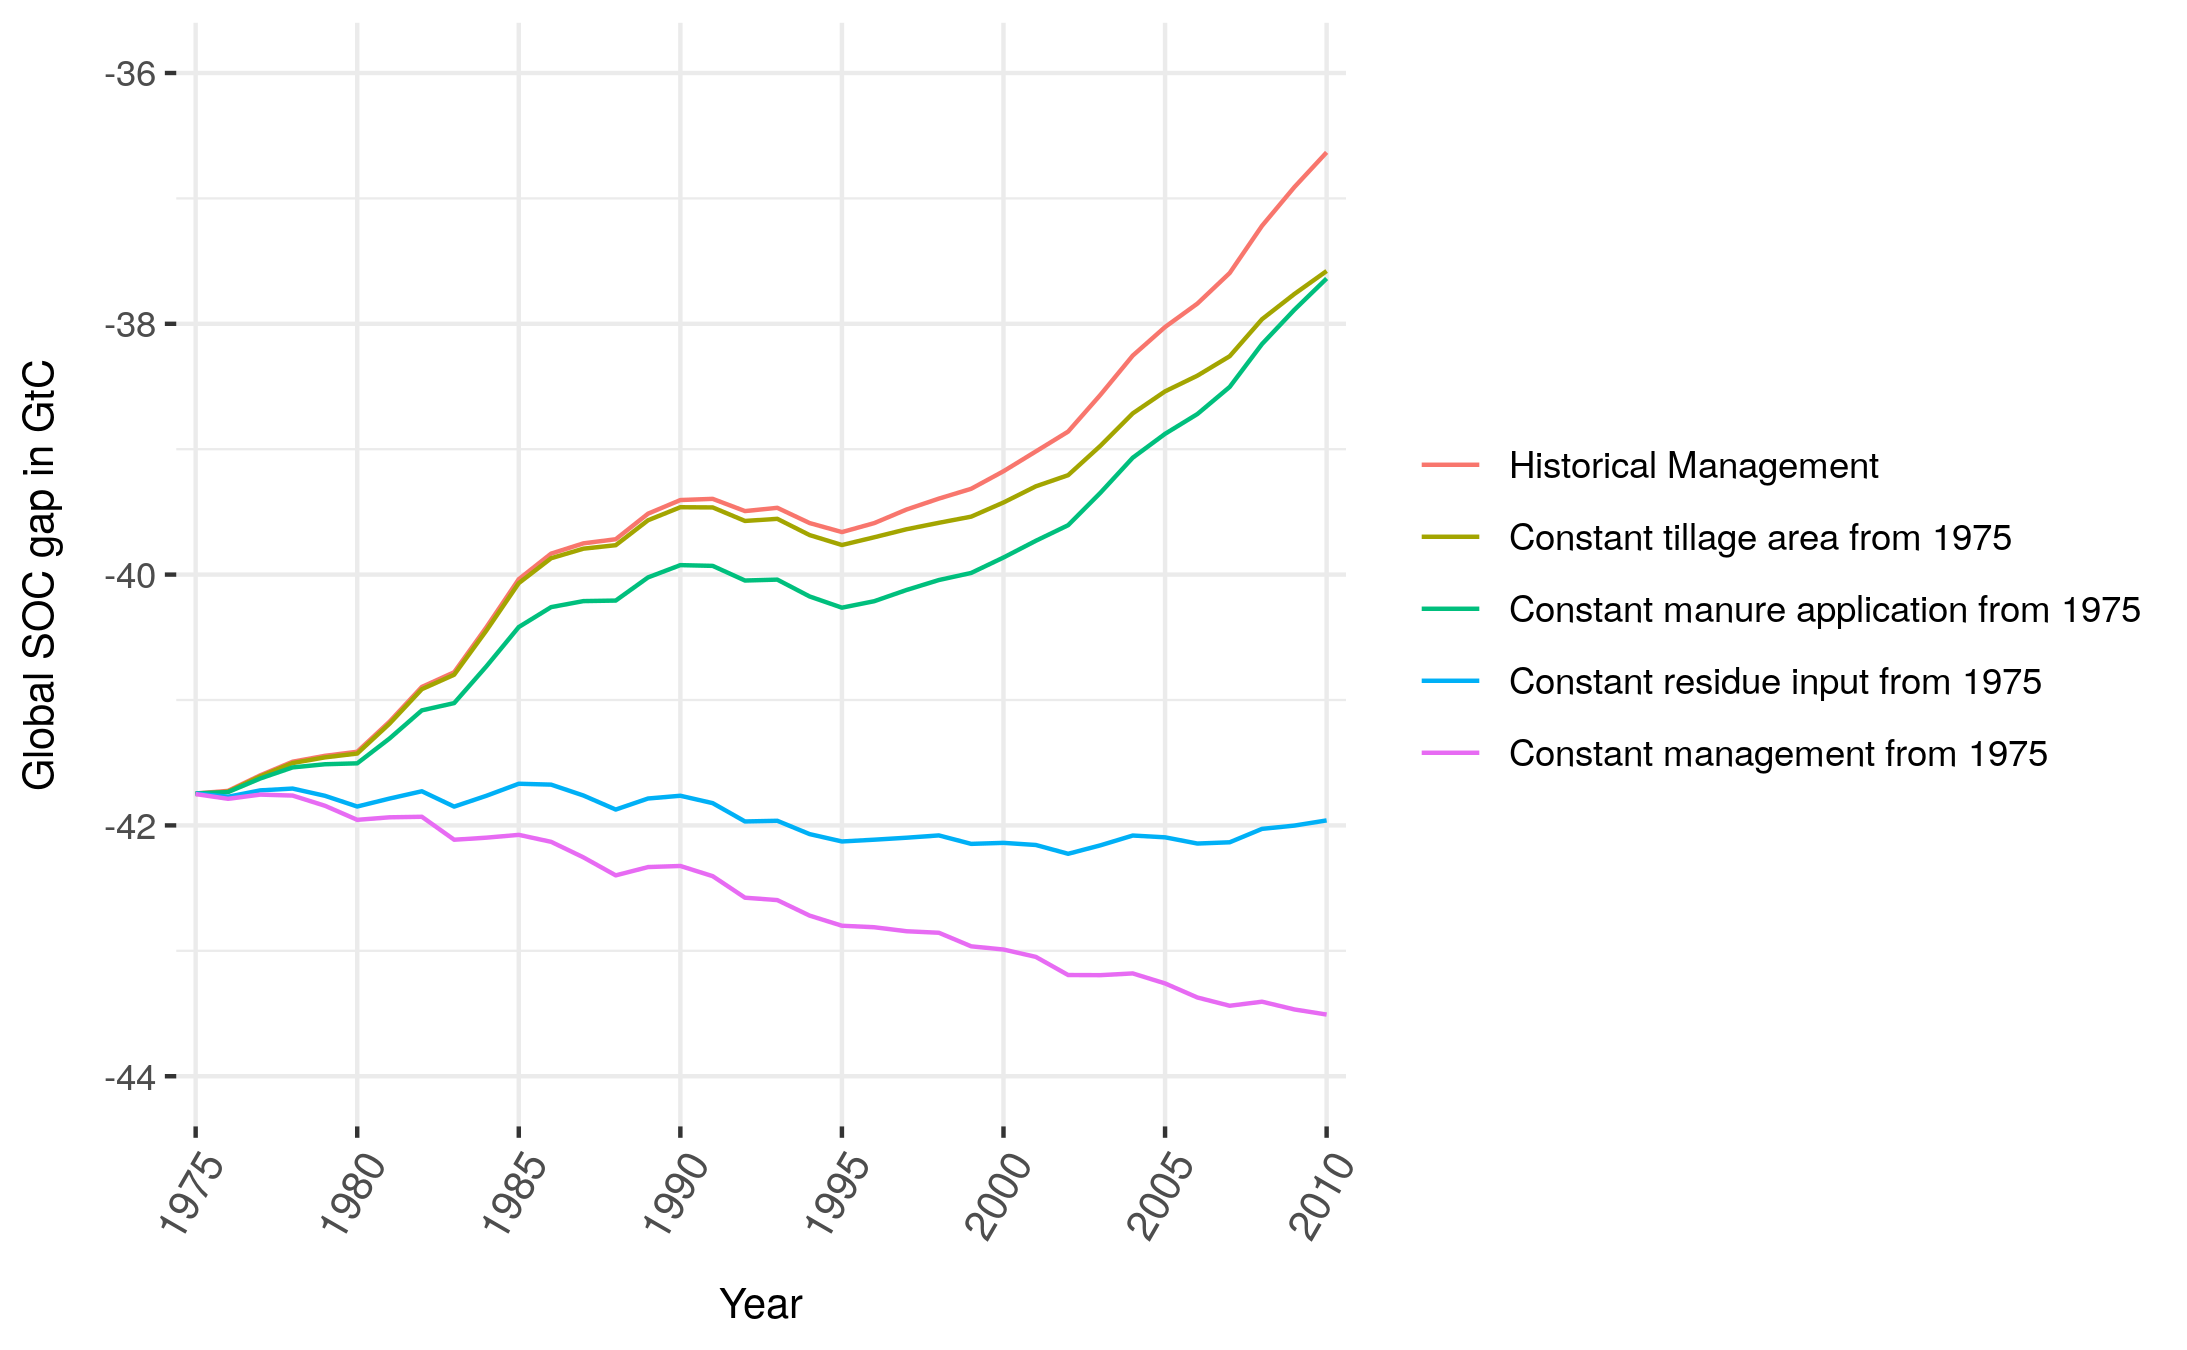
\includegraphics[width=18cm]{../ResultNotebooks/Output/Images/scenario} \caption{Global SOC gap in GtC for various stylized management counterfactual scenarios compared to the modeled historical baseline.}\label{fig:SOCscen}
\end{figure}

\begin{figure}[H]
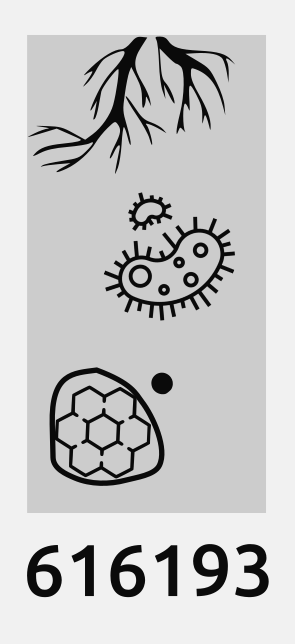
\includegraphics[width=16cm]{../ResultNotebooks/Output/Images/OuFlowFig} \caption{Global carbon flows (small numbers) and stocks (bold numbers) within the agricultural system for the year 2010 (in MtC): Most important carbon sources on cropland are crop residues. Note the two numbers on carbon inputs to soil denote carbon applied to the field and carbon entering the soil (difference is decomposed before official counting as soil).}\label{fig:FlowFig}
\end{figure}

\newpage

\newpage

\hypertarget{discussion}{%
\section{Discussion}\label{discussion}}

\hypertarget{including-agricultural-management-data-changes-the-sign-of-the-trend}{%
\subsection{Including agricultural management data changes the sign of the trend}\label{including-agricultural-management-data-changes-the-sign-of-the-trend}}

This study provides an analysis of historic SOC stock changes on cropland. We determine the SOC trends on cropland compared to a counterfactual scenario with a world under natural vegetation under identical historical climatic conditions (\(SOC_{natveg}\)). Our results show, that human activity lead to cumulative SOC emission of around 37 GtC in 2010. Whereas recent modelling estimates of global SOC emissions indicate an ongoing increase of SOC emissions (\citep{pugh_simulated_2015}, \citep{sanderman_soil_2017}), our study indicates that the global SOC gap is slowly closing due to improved management.

According to \citep{sanderman_soil_2017} cumulative SOC emissions since the beginning of human cropping activities have been at around 37 GtC for the first 30 cm of the soil with half of it attributed to grazing. Our estimate of 37 GtC in 2010 for cropland emissions only is twice as high as \citep{sanderman_soil_2017} estimations. However, there are large uncertainties in modelling SOC at the global scale, and the \citep{sanderman_soil_2017} results have been pointed out as potentially conservatively low compared with experimental results, leaving our results in an aceptable range.

Furthermore, \citep{sanderman_soil_2017} modelled historical trends based on agricultural land expansion without considering SOC variations due to different management systems at all. \citep{pugh_simulated_2015} considered management effects like tillage and residue recycling in a static way, but neither changes over time nor alignment to observed historical data like yields-levels or no-tillage areas were taken into account. The study moreover concludes that crop productivity gains (increasing yield levels by 18\%) do not lead to a~substantial decrease in SOC emissions, accounting for only less than 1\% change in SOC emissions.

Our study for the first time uses a dynamic management dataset as driver for SOC dynamics. We show that the moderate global cropland expansion of around 11\% between 1974 and 2010 and the resulting depletion of SOC stocks in converted cropland has been out weighted by improved agricultural yields and practices. This challenges \citep{pugh_simulated_2015} findings of only small effects due to improved practices.

Moreover, our sensitivity analysis indicates that (1) recycled residue biomass increases driven by higher yields as well as higher recycling rates play the most important role, followed by (2) improved manure recycling (e.g.~due to improved animal waste management systems) and (3) the adoption of no tillage practices.

Modelling management effects on the global scale comes however with parametric and structural uncertainties. As pointed out by \citep{keel_large_2017} and \citep{smith_how_2020}, carbon input calculations are highly sensitive to the choice of allometric functions determining below and above ground residue estimates from harvested quantities. \citep{keel_large_2017} question whether below ground residues might increase with a fixed root:shoot ratio rather than being independent of productivity gains. Moreover, the study pointed out that plant breeding shifts allometries which might not be reflected in outdated data sources. Following this line of argumentation, SOC results calculated in this study may overestimate actual SOC stocks due to an overestimation in residue biomass, for which the ratio compared to the harvested organ is normally reduced due to breeding. However, with an evaluation of management effects (see below), there is no indication for a systematic overrating of residue biomass. Rather, it is more likely that we are still missing carbon inputs to the soil.

\hypertarget{modeled-management-effect-in-line-with-default-ipcc-assumptions}{%
\subsection{Modeled management effect in line with default IPCC assumptions}\label{modeled-management-effect-in-line-with-default-ipcc-assumptions}}

To validate our modelled SOC stocks and stock changes under management, we compare our results to default IPCC stock changes factors (\citet{ipcc_2006_2006}, \citet{ipcc_2019_2019}) which are based on measurement data for croplands (see \ref{tab:SCFtable}). To allow for comparison, we aggregate our stock change factors to the four IPCC climate zones.

\begin{figure}
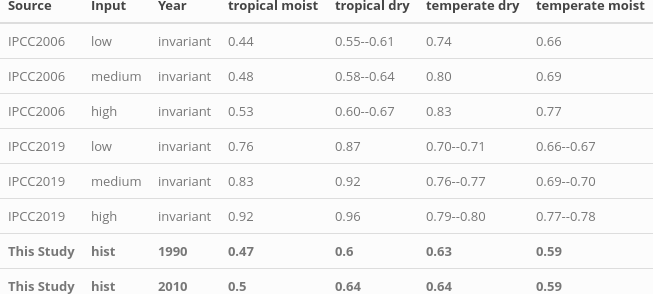
\includegraphics[width=16cm]{../ResultNotebooks/Output/Images/TableSCF_comparison} \caption{This table shows different estimates of stock change factors $F_{SCF}$, defined as the SOC stock of managed croplands relative to the counterfactual SOC stock of undisturbed natural vegetation. We compare average values for four IPCC climate zone classifications. IPCC 2006 and 2019 default factors (medium input) as well as altered factors for low input of organic matter without any other subsystem consideration are compared to results for 1990 and 2010 of this study (SOC budget).}\label{fig:SCFtable}
\end{figure}

Our estimates correspond very well to the default stock-change factors used for the tier 1 estimation of IPCC, 2006. For the tropical regions the assumptions changed notably from the guidelines in 2006 to the update in 2019, leaving our results too low in comparison with IPCC, 2019. Considering yield gaps in mainly developing regions in the tropics the default assumption of medium input systems might be an overestimation of actual SOC state. The additional effect of considering low inputs of biomass in tropical regions can however not explain the full mismatch to IPCC 2019 values but account for 14-21\% of it.

With regard to the time trend, our study shows the substantial impact of changing management factors on the development of \(F_{SCF}\).

\hypertarget{soc-stocks-inline-with-literature}{%
\subsection{SOC stocks inline with literature}\label{soc-stocks-inline-with-literature}}

The world's SOC stock and its changes are highly uncertain (cite), which is seen in the wide range of global SOC stock estimates (see \ref{tab:SOCtable}).

\begin{figure}[H]
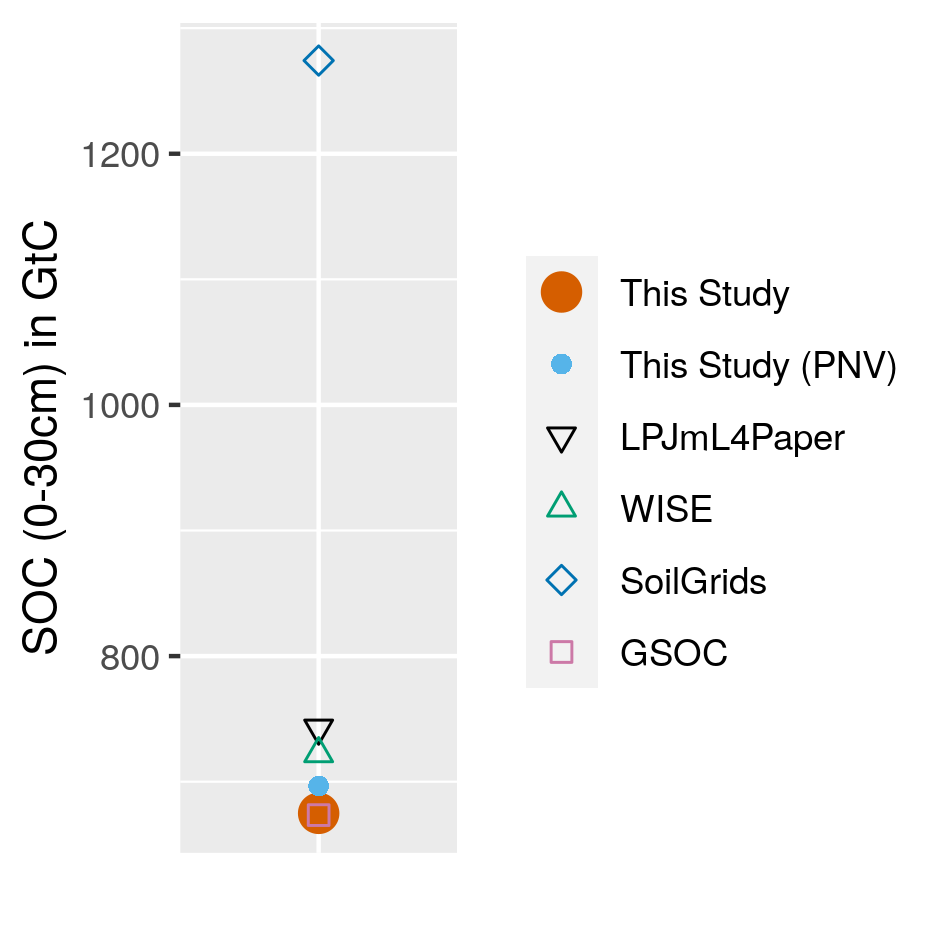
\includegraphics[width=8cm]{../ResultNotebooks/Output/Images/glo_comparisonfigure} \caption{Modelled as well as data based estimation for global SOC stock in GtC for the first 30 cm of soil aggregated over all land area. Note that SoilGrids, GSOC and WISE do not consider changes over time and rely on soil profile data gather over a long period of time, which makes it hard to pinpoint a specific year for these SOC estimations. In this context they will be compared to modelled data (LPJmL4, this study) for the year 2010.}\label{fig:SOCtable}
\end{figure}

The global estimates of SOC stock from this study are on the lower end compared to other modelled results or more data driven estimates. Looking at regional results \ref{append:regcompare}, our estimates turn out to be in good agreement for most regions, with the largest deviations for boreal areas. Considering that the model was parametrized for croplands, these mismatches are not~suprising as the temperature effects on decomposition are fundamentally different for permafrost soils. To avoid that this bias influences our results, our study focuses exclusively on cropland soils, excluding most of the boreal zone. Moreover, when focussing on SOC changes on cropland, pristine natural vegetated areas without human land management under the same historic climatic conditions cancel out in the calculation of SOC emissions.

Our estimates for total SOC stocks of the world, as well as our SOC initialization, are dominated by the representation of natural lands and pastures, which are however only estimated in a basic manner. For example, we do not have a differentiated parametrization of nitrogen and lignin content of litterfall for woody and grass type biomes. This leaves carbon inputs and decay behavior for natural land and pastures rather uncertain. The absolute values of stocks and emissions from land-use change therefore have to be used with caution. Especially in less forested areas the natural land representation higher uncertainty may arise from the parametrization assumptions of natural litterfall.

Nevertheless, total SOC stocks are in a reasonable range and results for SOC stock changes in relative or absolute numbers are not altered by pristine vegetated areas at all. The SOC gap from changed management is only affected by the natural vegetation representation in the case of land use transitions. In this case, former natural land SOC stocks decline. However, as pointed out before, due to low cropland expansion rates, land use change-related SOC declines are outweighed by the general trend of increasing SOC stocks on existing cropland due to management improvements.
We conducted a sensitivity analysis for a wide range of possible parameter combinations for lignin and nitrogen parametrization of natural litterfall, which tend to change the global SOC stock substantially for different choices
(see appendix). This shows that the general trend of decreasing SOC gap is not altered even under very high estimates for natural SOC stocks.

\hypertarget{important-shortcomings-might-be-added-as-well}{%
\subsection{Important shortcomings --\textgreater{} might be added as well}\label{important-shortcomings-might-be-added-as-well}}

The \textbf{initialization of SOC stocks} in 1960 is assumed to be in steady state considering the land use pattern and management effects of the initialization year followed by a run-in period of 15 years, till the analysis of the results start. That is inline with IPCC guidelines calling for a run-in period of 5-20 years. However, the results are heavily influenced by it as \ref{append:initcompare} suggested. Not only the level of the SOC gap is shifted, also the declining trend is much smaller or even not visible at all anymore. For the artificial assumption of starting with potential natural vegetation in 1961 the SOC gap is fluctuating around 10 GtC for the period 1975--2010. For the more moderate assumption, that half of the transition towards the steady-state under land use has already appeared in 1960, the SOC gap is around 23 GtC in 2010. The relative declining trend for the SOC gap between 1975 and 2010 (-12\%) is however almost the same as for our historic estimation (-14\%). According to LUH \citep{hurtt_harmonization_2020} cropland area has increased over 62\% since 1900 leaving our choice of initialization values too low, since reaching a new steady-state can take decades or even centuries. Having no yield or management data available before our initialization year leaves us with imperfect initialization knowledge, where our initialization choice is probably closer to real world values than starting from a natural vegetated steady-state.

Following the IPCC guidelines this study has limited its focus to the \textbf{first 30 cm of the soil profile}. In this regard several aspects are over simplified within our approach. Firstly, distribution of carbon inputs into different soil layers are neglected and all carbon inputs are allocated to the topsoil. This particularly overestimates SOC stocks in the first 30 cm of soil below deeper rooting vegetation, which is certainly the case for most of the woody natural vegetated areas. Consequently, our SOC loss estimates are too high.
Secondly changes to the subsoil due to tillage are neglected, which might be important to noticed, hence studies (see Don on tillage) have shown, the subsoil to be a game changer in evaluating total SOC losses or gains for no-tillage systems. It has been argued that for intensively tilled soils, subsoil SOC is increasing due to the import of carbon rich topsoil to deeper soil layers. Following this arguments SOC stocks in croplands might even be underestimated.

Carbon displacement via \textbf{leaching and erosion} is neglected in this study. As pointed out by several studies (cite), the final fate of leached or eroded carbon is uncertain. Whereas for soil quality analysis SOC displacement might play an important role, in this budget approach focusing especially on SOC emissions, displaced but not emitted SOC can be treated as SOC stayed on croplands.
\newpage

\conclusions

Outlook including perspective on mitigation (and soc enhancement in the future).
\newpage

\hypertarget{appendix}{%
\section{Appendix}\label{appendix}}

\hypertarget{append:subsection2mrfunctions}{%
\subsection{table on method subsections to functions within R packages}\label{append:subsection2mrfunctions}}

\hypertarget{append:Tableluh2fao2mag}{%
\subsection{table on mapping LUH2FAO2MAG}\label{append:Tableluh2fao2mag}}

\hypertarget{append:Tablekcr2kres}{%
\subsection{kcr2kres mapping}\label{append:Tablekcr2kres}}

\hypertarget{append:Tablec2dm}{%
\subsection{carbon 2 dry matter}\label{append:Tablec2dm}}

Litter is coming from LPJmL in carbon units - transformation with 0.44 is done twice reverting the effect of the transformation

\hypertarget{append:TableclossAWMS}{%
\subsection{closs in AWMS - Table}\label{append:TableclossAWMS}}

\hypertarget{append:climatemap}{%
\subsection{map on climate zone used for SCF}\label{append:climatemap}}

\hypertarget{append:regcompare}{%
\subsection{regional SOC stock in GtC from different sources}\label{append:regcompare}}

\begin{figure}[H]
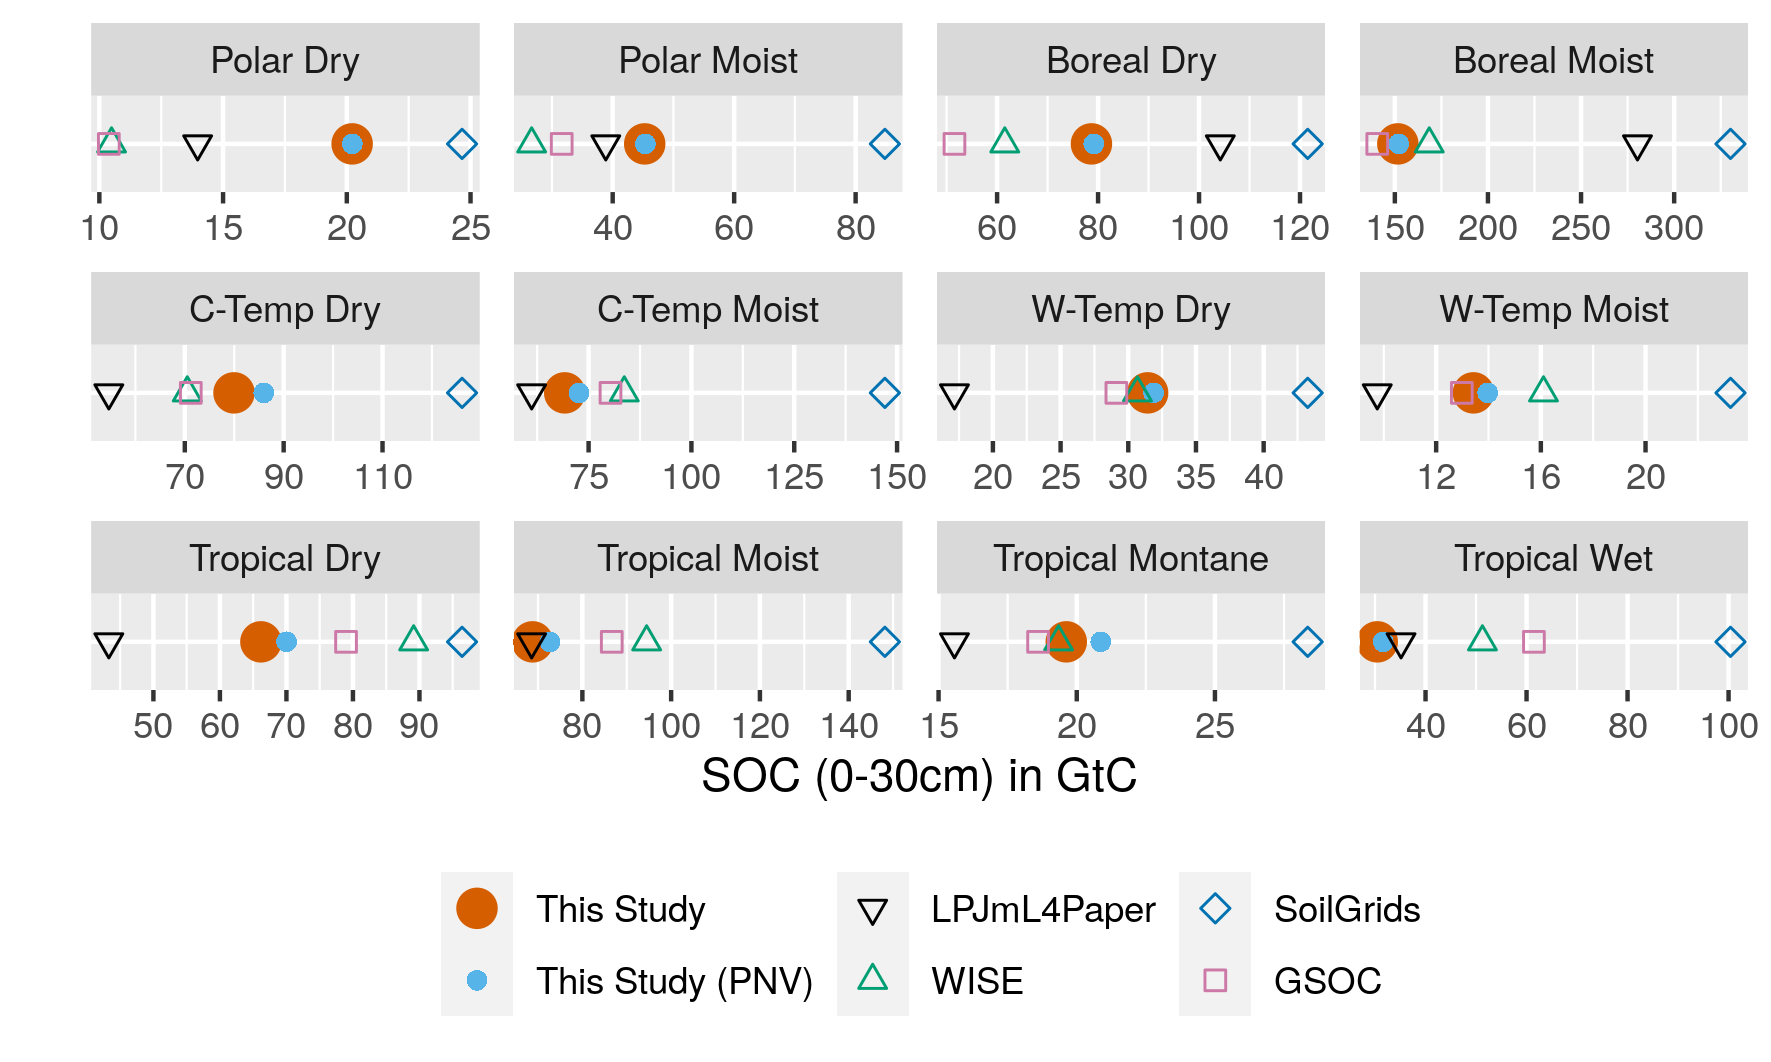
\includegraphics[width=1\linewidth]{../ResultNotebooks/Output/Images/reg_comparisonfigure} \caption{Modelled as well as data based estimation for global SOC stock in GtC for the first 30 cm of soil aggregated over all land area. Note that SoilGrids, GSOC and WISE do not consider changes over time and rely on soil profile data gather over a long period of time, which makes it hard to pinpoint a specific year to these SOC estimations. In this context they will be compared to modelled data (LPJmL4, this study) for the year 2010.}\label{fig:regSOCtable}
\end{figure}

\hypertarget{append:initcompare}{%
\subsection{global SOC gap in GtC for different initialization choices}\label{append:initcompare}}

\begin{figure}[H]
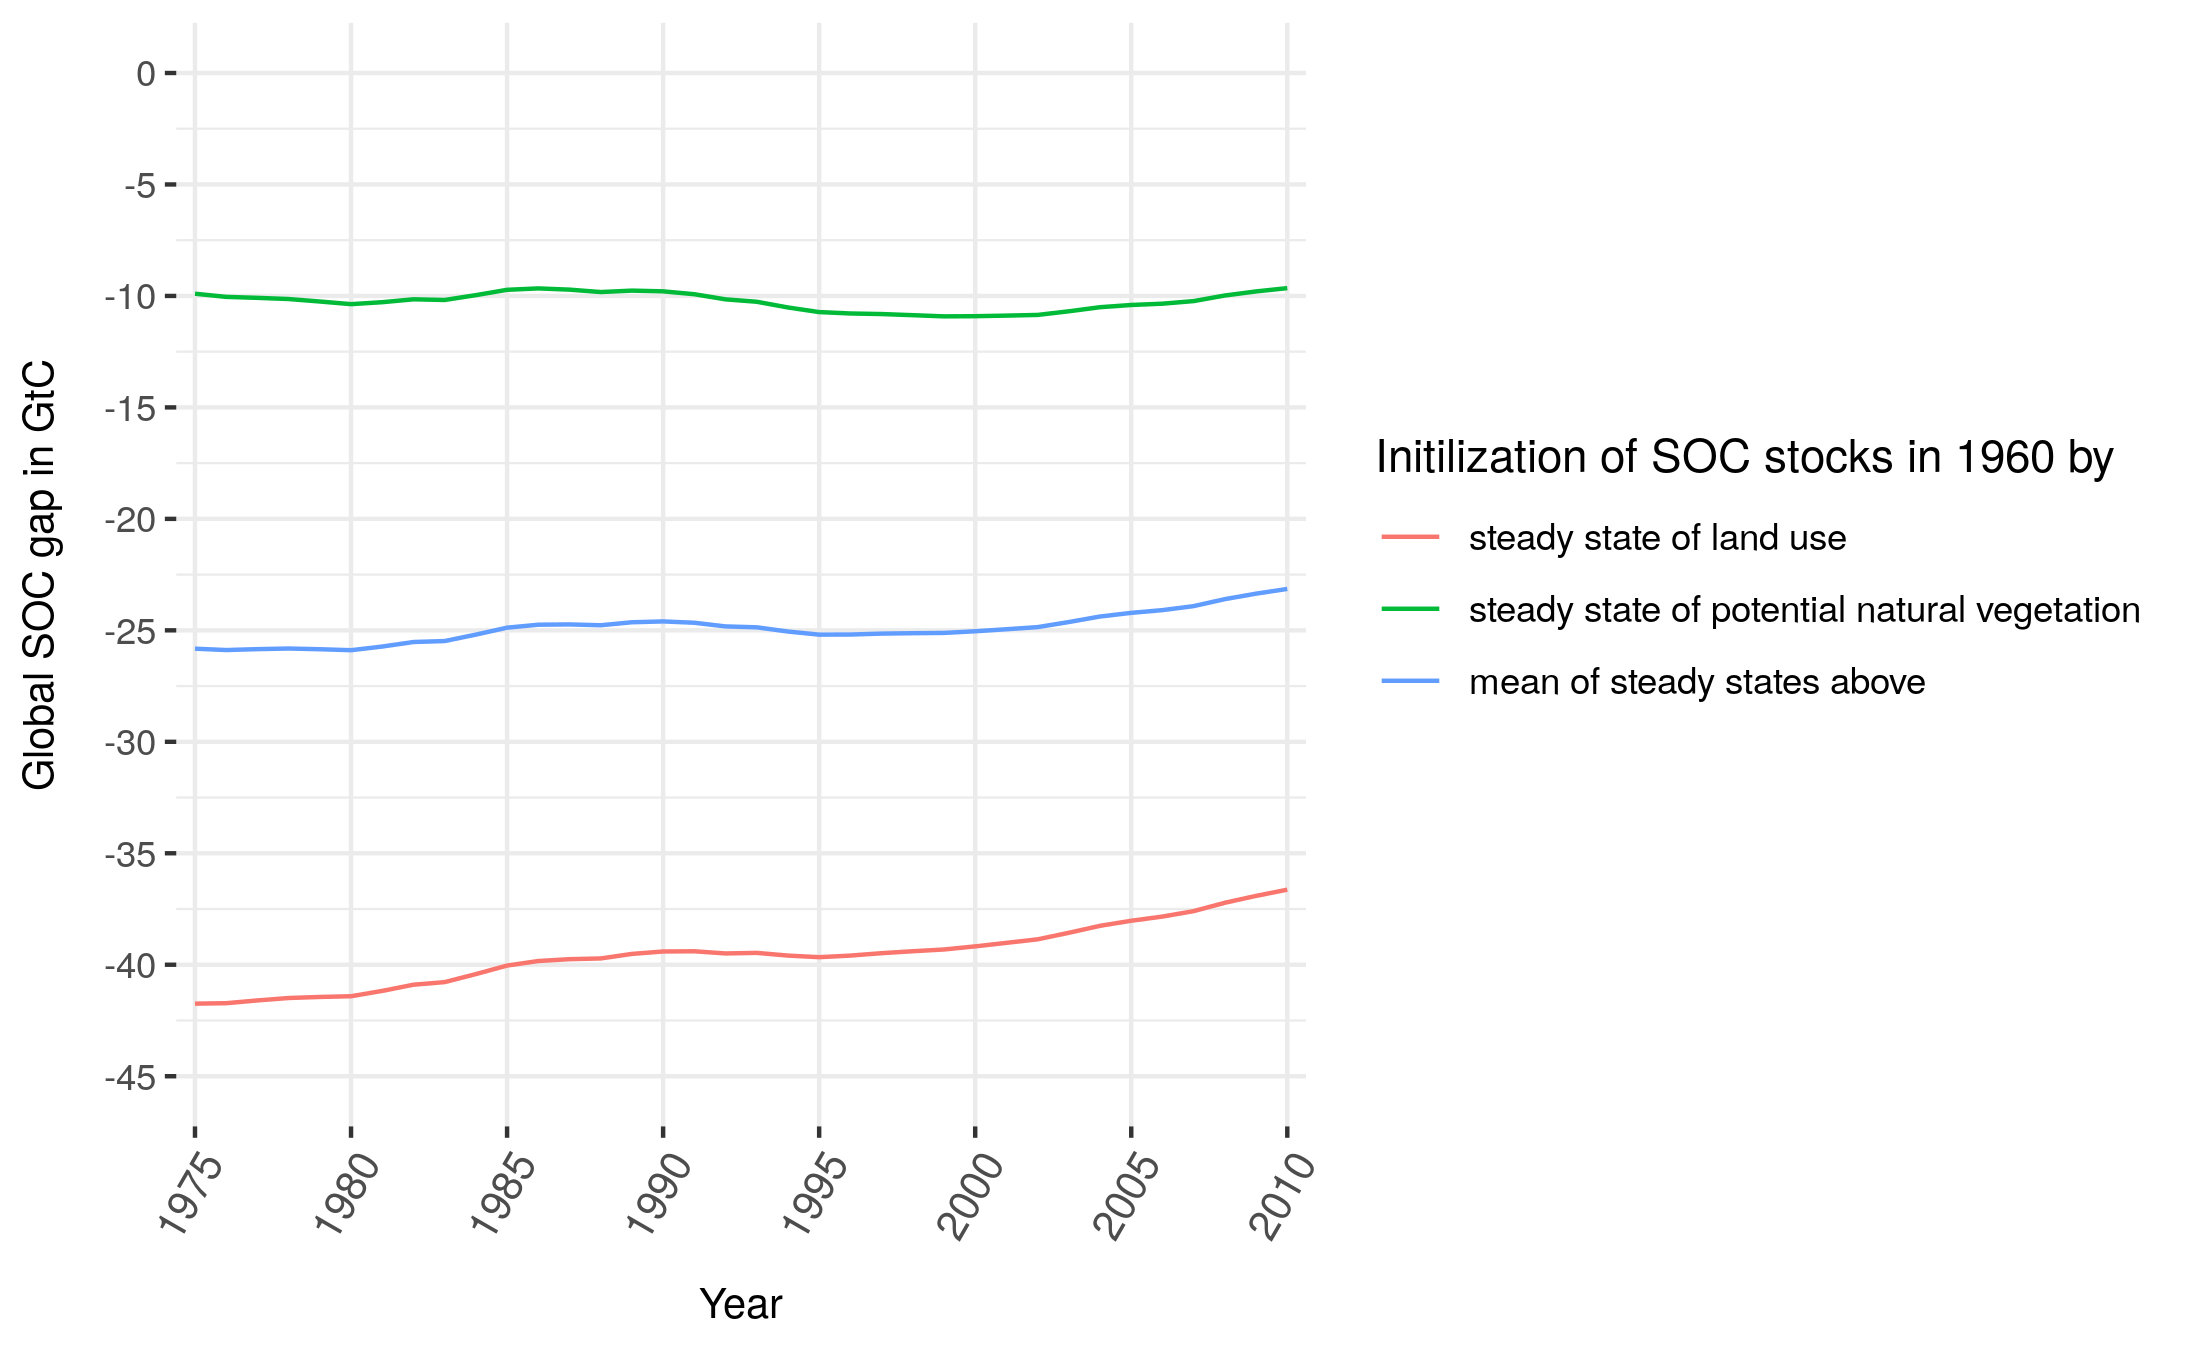
\includegraphics[width=1\linewidth]{../ResultNotebooks/Output/Images/scenario_lu} \caption{Global SOC gap in GtC for the first 30 cm of soil for different initialization choices.}\label{fig:initSOC}
\end{figure}

\hypertarget{more-short-comings}{%
\subsection{more short comings}\label{more-short-comings}}

\begin{itemize}
\item
  Fertilizer interaction is not included here by accounting for additional N supply that would alter C:N ratio of the carbon inputs. Tier 2 steady-state method is neglecting fertilizer application, however we would have fertilizer amounts at hand to include them, if proper representation of fertilizer within the method would be possible to add.
\item
  Pasture dynamics are neglected and treated as natural vegetation, which might be -- looking on pasture degradation due to overgrazing -- oversimplified for some spots, but is inline with assumption on pasture SOC stocks done before (see Tier 1 IPCC). (Note that also manure excreted to as well as tillage on pastures are neglected within this analysis, since we focus purely on cropland dynamics.)
\item
  Irrigated areas are not crop specific and irrigation is not restricted to growing periods (since it is very complex to calculate average growing periods). Crop specific growing periods might be possible using LPJmL data.
\item
  Flooded rice area are not represented correctly as parametrization does not hold true for flooded conditions.
\item
  Non-net/Gross land use transitions are not tracked in this study.
\item
  Within cropland we do not track croparea transitions, but rather look at statistical distributions of the crop functional types. Due to crop rotations and missing data on crop specific distributions, these transitions would be any way rather uncertain.
\item
  The disaggregation of manure to build-up areas (in the case of extensive monogastrics) is leading to a lot of displaced manure (?) that is cut off
\item
  It is known that there are mismatches between FAO statistics and LUH areas. As far as possibles there were harmonized within this study.
  \newpage
\end{itemize}




\codedataavailability{Software code for paper and result prepartion can be found under www.github.com/k4rst3ns/. Data used for the output can be found under .} %% use this section when having data sets and software code available



%%%%%%%%%%%%%%%%%%%%%%%%%%%%%%%%%%%%%%%%%%
%% optional

%%%%%%%%%%%%%%%%%%%%%%%%%%%%%%%%%%%%%%%%%%

%%%%%%%%%%%%%%%%%%%%%%%%%%%%%%%%%%%%%%%%%%
\authorcontribution{Karstens wrote code and paper build on work of Bodirsky (and ).
Bodirsky, and Popp revised paper.} %% optional section

%%%%%%%%%%%%%%%%%%%%%%%%%%%%%%%%%%%%%%%%%%
\competinginterests{The authors declare no competing interests.} %% this section is mandatory even if you declare that no competing interests are present

%%%%%%%%%%%%%%%%%%%%%%%%%%%%%%%%%%%%%%%%%%
\disclaimer{We like Copernicus.} %% optional section

%%%%%%%%%%%%%%%%%%%%%%%%%%%%%%%%%%%%%%%%%%
\begin{acknowledgements}
Thanks to the rticles contributors!
\end{acknowledgements}

%% REFERENCES
%% DN: pre-configured to BibTeX for rticles

%% The reference list is compiled as follows:
%%
%% \begin{thebibliography}{}
%%
%% \bibitem[AUTHOR(YEAR)]{LABEL1}
%% REFERENCE 1
%%
%% \bibitem[AUTHOR(YEAR)]{LABEL2}
%% REFERENCE 2
%%
%% \end{thebibliography}

%% Since the Copernicus LaTeX package includes the BibTeX style file copernicus.bst,
%% authors experienced with BibTeX only have to include the following two lines:
%%
\bibliographystyle{copernicus}
\bibliography{SOCbudget2.bib}
%%
%% URLs and DOIs can be entered in your BibTeX file as:
%%
%% URL = {http://www.xyz.org/~jones/idx_g.htm}
%% DOI = {10.5194/xyz}


%% LITERATURE CITATIONS
%%
%% command                        & example result
%% \citet{jones90}|               & Jones et al. (1990)
%% \citep{jones90}|               & (Jones et al., 1990)
%% \citep{jones90,jones93}|       & (Jones et al., 1990, 1993)
%% \citep[p.~32]{jones90}|        & (Jones et al., 1990, p.~32)
%% \citep[e.g.,][]{jones90}|      & (e.g., Jones et al., 1990)
%% \citep[e.g.,][p.~32]{jones90}| & (e.g., Jones et al., 1990, p.~32)
%% \citeauthor{jones90}|          & Jones et al.
%% \citeyear{jones90}|            & 1990

\end{document}
